%iffalse
\let\negmedspace\undefined
\let\negthickspace\undefined
\documentclass[journal,12pt,onecolumn]{IEEEtran}
\usepackage{cite}
\usepackage{amsmath,amssymb,amsfonts,amsthm}
\usepackage{algorithmic}
\usepackage{graphicx}
\usepackage{textcomp}
\usepackage{xcolor}
\usepackage{txfonts}
\usepackage{listings}
\usepackage{enumitem}
\usepackage{mathtools}
\usepackage{pgfplots}
\usepackage{gensymb}
\usepackage{circuitikz}
\usepackage{comment}
\usepackage[breaklinks=true]{hyperref}
\usepackage{tkz-euclide} 
\usepackage{listings}
\usepackage{gvv}                                        
%\def\inputGnumericTable{}                                 
\usepackage[latin1]{inputenc}                                
\usepackage{color}                                            
\usepackage{array}                                            
\usepackage{longtable}                                       
\usepackage{calc}                                             
\usepackage{multirow}                                         
\usepackage{hhline}                                           
\usepackage{ifthen}                                           
\usepackage{lscape}
\usepackage{tabularx}
\usepackage{array}
\usepackage{float}

\usepackage{enumitem}
\usepackage{xcolor}
%\usepackage{multicol}


\newtheorem{theorem}{Theorem}[section]
\newtheorem{problem}{Problem}
\newtheorem{proposition}{Proposition}[section]
\newtheorem{lemma}{Lemma}[section]
\newtheorem{corollary}[theorem]{Corollary}
\newtheorem{example}{Example}[section]
\newtheorem{definition}[problem]{Definition}
\newcommand{\BEQA}{\begin{eqnarray}}
\newcommand{\EEQA}{\end{eqnarray}}
\newcommand{\define}{\stackrel{\triangle}{=}}
\theoremstyle{remark}
\newtheorem{rem}{Remark}

\title{2017-EE-1-13}
\author{AI24BTECH11023 - Tarun Reddy Pakala}
\begin{document}
\bibliographystyle{IEEEtran}

\maketitle
\bigskip
\renewcommand{\thefigure}{\theenumi}
\renewcommand{\thetable}{\theenumi}
\begin{enumerate}
\item The matrix \textbf{A}=$
\begin{bmatrix}
\frac{3}{2} & 0 & \frac{1}{2} \\
0 & -1 & 0 \\
\frac{1}{2} & 0 & \frac{3}{2}
\end{bmatrix}
$ has three distinct eigenvalues and one of its eigenvectors is $
\begin{bmatrix}
1  \\
0  \\
1 
\end{bmatrix}
$. Which one of the following can be another eigenvector of \textbf{A}?
\begin{enumerate}
    \item $
\begin{bmatrix}
0  \\
0  \\
-1 
\end{bmatrix}
$
    \item $
\begin{bmatrix}
-1  \\
0  \\
0
\end{bmatrix}
$
    \item $
\begin{bmatrix}
1 \\
0  \\
-1 
\end{bmatrix}
$
    \item $
\begin{bmatrix}
1  \\
-1  \\
1 
\end{bmatrix}
$
\end{enumerate}
\item For a complex number $z,\;\lim_{z\to i}\frac{z^2+1}{z^3+2z-1\brak{z^2+2}}$ is
\begin{enumerate}
    \item $-2i$
    \item $-i$
    \item $i$
    \item $2i$
\end{enumerate}
\item Let $z\brak{t}=x\brak{t}*y\brak{t}$ where "*" denotes convolution. Let $c$ be a positive real-valued constant. Choose the correct expression for $z\brak{ct}$. 
\begin{enumerate}
    \item $c\cdot x\brak{ct}*y\brak{ct}$
    \item $x\brak{ct}*y\brak{ct}$
    \item $c\cdot x\brak{t}*y\brak{ct}$
    \item $c\cdot x\brak{ct}*y\brak{t}$
\end{enumerate}
\item A solid iron cylinder is placed in a region containing a uniform magnetic field such that the cylinder axis is parallel to the magnetic field direction. The magnetic field lines inside the cylinder will
\begin{enumerate}
    \item bend closer to the cylinder 
    \item bend farther away from the axis
    \item remain uniform as before 
    \item cease to exist inside the cylinder
\end{enumerate}
\item Consider an electron, a neutron and a proton initially at rest and placed along a straight line such that the neutron is exactly at the center of the line joining the electron and proton. At $t=0$, the particles are released but are constrained to move along the same straight line. Which of these will collide first? 
\begin{enumerate}
    \item the particles will never collide
    \item all will collide together
    \item proton and neutron
    \item electron and neutron
\end{enumerate}
\item The transfer function of a system is given by. $$\frac{V_o\brak{s}}{V_i\brak{s}}=\frac{1-s}{1+s}$$ Let the output of the system be $v_o\brak{t}=V_m\sin\brak{\omega t+\phi}$ for the input, $v_i\brak{t}=V_m\sin \brak{\omega t}$. Then the minimum and maximum values of $\phi$ \brak{\text{in radius}} are respectively
\begin{enumerate}
    \item $\frac{-\pi}{2}$ and $\frac{\pi}{2}$
    \item $\frac{-\pi}{2}$ and $0$
    \item $0$ and $\frac{\pi}{2}$
    \item $-\pi$ and $0$
\end{enumerate}
\item Consider the system with following input-output relation $$y\sbrak{n}=\brak{1+\brak{-1}^n}x\sbrak{n}$$ where, $x\sbrak{n}$ is the input and $y\sbrak{n}$ is the output. The system is
\begin{enumerate}
    \item invertible and time invariant 
    \item invertible and time varying
    \item non-invertible and time invariant
    \item non-invertible and time varying
\end{enumerate}
\item A $4$ pole induction machine is working as an induction generator. The generator supply frequency is $60\;Hz$. The rotor current frequency is $5\;Hz$. The mechanical speed of the rotor in $RPM$ is
\begin{enumerate}
    \item $1350$
    \item $1650$
    \item $1950$
    \item $2250$
\end{enumerate}
\item A source is supplying a load through a 2-phase, 3-wire transmission system as shown in the figure below. The instantaneous voltage and current in phase are $v_{an}=220\sin{\brak{100\pi t}}\;V$ and $i_a=10\sin{\brak{100\pi t}}\;A$, respectively. Similarly for phase-b, the instantaneous voltage and current are $v_{bn}=220\cos{\brak{100\pi t}}\;V$ and $i_b=10\cos{\brak{100\pi t}}\;A$, respectively.
%input for figure 1
	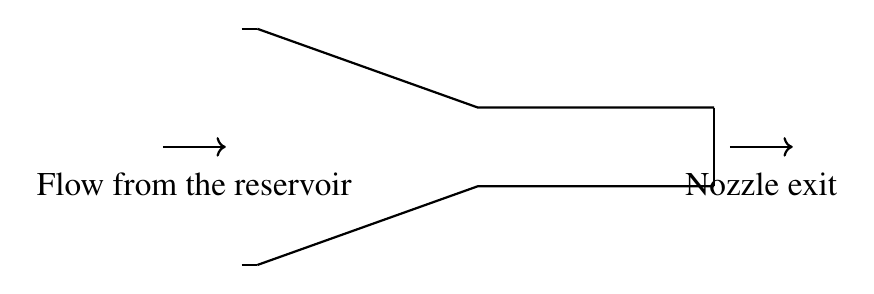
\begin{tikzpicture}
    % Draw the nozzle shape with short vertical lines at the opening
    \draw[thick] (-3,1.5) -- (-2.8,1.5);
    \draw[thick] (-3,-1.5) -- (-2.8,-1.5);
    \draw[thick] (-2.8,1.5) -- (0,0.5) -- (3,0.5);
    \draw[thick] (-2.8,-1.5) -- (0,-0.5) -- (3,-0.5);
    
    % Vertical line at the nozzle exit
    \draw[thick] (3,0.5) -- (3,-0.5);

    % Flow direction arrows
    \draw[->, thick] (-4,0) -- (-3.2,0);
    \draw[->, thick] (3.2,0) -- (4,0);

    % Labels for the flow and nozzle exit, placed below arrows
    \node[below] at (-3.6,-0.2) {\large Flow from the reservoir};
    \node[below] at (3.6,-0.2) {\large Nozzle exit};
\end{tikzpicture}

	\begin{enumerate}
    \item $2200\;W$
    \item $2200\sin^2{\brak{100\pi t}}\;W$
    \item $4400\;W$
    \item $2200\sin{\brak{100\pi t}}\cos{\brak{100\pi t}}\;W$
\end{enumerate}
\item A 3-bus power system is shown in the figure below, where the diagonal element of $Y$-bus matrix are:$Y_{11}=-j12\;pu,\;Y_{22}=-j\;pu$ and $Y_{33}=-j7\;pu$.\\
%input for figure 2
	\begin{figure}[!ht]
\centering
\resizebox{3cm}{3cm}{%
\begin{circuitikz}
\tikzstyle{every node}=[font=\LARGE]
\draw [ line width=0.6pt](2.75,12) to[sinusoidal voltage source, sources/symbol/rotate=auto] (3.25,11.5);
\draw [ line width=0.6pt](3.25,11.75) to[european resistor] (9.5,11.75);
\draw [line width=0.6pt, ->, >=Stealth] (9.5,11.75) -- (9.5,11);
\draw [ line width=0.6pt](4,12.25) to[short] (4,11.25);
\draw [ line width=0.6pt](4,11.5) to[short] (4,11);
\draw [ line width=0.6pt](8.75,12.25) to[short] (8.75,11);
\draw [ line width=0.6pt](4,11.25) to[short] (4.5,11.25);
\draw [ line width=0.6pt](8.75,11.25) to[short] (8.25,11.25);
\draw [ line width=0.6pt](4.25,11.25) to[short] (5.25,11.25);
\draw [ line width=0.6pt](8.25,11.25) to[short] (7.25,11.25);
\draw [ line width=0.6pt](5,11.25) to[european resistor] (5,8.5);
\draw [ line width=0.6pt](7.5,11.25) to[european resistor] (7.5,8.5);
\draw [ line width=0.6pt](4.75,8.5) to[short] (8,8.5);
\draw [line width=0.6pt, ->, >=Stealth] (6.25,8.5) -- (6.25,7.75);
\node [font=\normalsize] at (6.75,8) {Bus 3};
\node [font=\normalsize] at (4,12.5) {Bus 1};
\node [font=\normalsize] at (8.75,12.5) {Bus 2};
\node [font=\normalsize] at (6.25,12.25) {j q};
\node [font=\normalsize] at (4.5,10) {j r};
\node [font=\normalsize] at (8.25,9.75) {j p};
\end{circuitikz}
}%

\label{fig:my_label}
\end{figure}

The per unit values of the line reactances $p,q$ and $r$ shown in the figure are
\begin{enumerate}
    \item $p=-0.2,\;q=-0.1,\;r=-0.5$
    \item $p=0.2,\;q=0.1,\;r=0.5$
    \item $p=-5,;q=-10,\;r=-2$
    \item $p=5,\;q=10,\;r=2$
\end{enumerate}
\item A closed loop system has the characteristic equation given by $s^3+Ks^2+\brak{K+2}s+3=0$. For this system to be stable, which one of the following conditions should be satisfied?
\begin{enumerate}
    \item $0\;<\;K\;<\;0.5$
    \item $0.5\;<\;K\;<\;1$
    \item $0\;<\;K\;<\;1$
    \item $K\;>\;1$
\end{enumerate}
\item The slope and level detector circuit in a $CRO$ has a delay of $100\;ns$. The start-stop sweep generator has a response time of $50\;ns$. In order to display correctly, a delay line of 
\begin{enumerate}
    \item $150\;ns$ has to be inserted into the $y$-channel
    \item $150\;ns$ has to be inserted into the $x$-channel
    \item $150\;ns$ has to be inserted into both $x$ and $y$ channels
    \item $100\;ns$ has to be inserted into both $x$ and $y$ channels
\end{enumerate}
\item The Boolean expression $AB+A\Bar{C}+BC$ simplifies to 
\begin{enumerate}
    \item $BC\;+A\Bar{C}$
    \item $AB\;+\;A\Bar{C}\;+\;B$
    \item $AB\;+\;A\Bar{C}$
    \item $AB\;+\;BC$
\end{enumerate}

\end{enumerate}
\end{document}
